\documentclass[11pt]{article}

\usepackage{listings}
\usepackage{verbatim}
\usepackage{amsmath}
\usepackage{float}
\usepackage{hyperref}
\usepackage{graphicx}



\lstset{
	breaklines=true,
	tabsize=2,
	language=C,
  	showstringspaces=false,
	basicstyle=\footnotesize\ttfamily,
%	keywordstyle=\bfseries\color{green!40!black},
%	commentstyle=\itshape\color{purple!40!black},
%	identifierstyle=\color{blue},
%	stringstyle=\color{orange}
}

\begin{document}
\title{Parallel Computing\\184.710\\Group 5 Projects}
\author{Peter Neubauer\\ 0725263 \and Bruno Pfeiffer \\ 0717311}
\date{\today}
\maketitle
\newpage
\tableofcontents

\newpage
\section{Introduction}

The entire project consists of the subprojects OMP project one, two and three, Cilk project one and MPI project one, two and three. All project files (code, Makefiles, scripts, R files) and results can be found here:

\begin{center}
\url{http://GIT LINK}

\url{http://DROPBOX LINK}
\end{center}

For all tests, we employed a deterministic number generator in various configurations that provided numbers based on the following conditions, given an $upper$ and $lower$ bound:
\begin{enumerate}
\item Powers of 2 $ \in [lower, upper]$
\item Prime numbers $\in [lower, upper]$, at most fifty for a single query
\item Single digits, appended by trailing zeros $\in [lower, upper]$, meaning numbers of the form: \verb=[1-9]0*=
\end{enumerate}
All tests were performed on Jupiter and Saturn. During testing, we noticed that performance was poor in several circumstances due to other processes disturbing the execution.

\newpage
\section{OpenMP: Prefix Sums}
For this project, we decided to implement an OpenMP program as opposed to a pthread implementation. We chose this particular option due to the simpler handling of OpenMP. All three parallel algorithms have been programmed in separate programs, each according to the guidelines found in the lecture script. The data type was generified using a C defintion ($ATYPE$). The programs accepts the arguments ($n, t$) to set the size of the problem and number of threads to be used.
All programs (save the sequential reference implementation) use \emph{Performance Counters} to track work:

\begin{description}
\item[Operation Counter] Counts only the '$+$' operations used in the prefix sums. 
\item[Access Counter] Counts every single array access (read AND write).
\end{description}

We found that all algorithms showed similar performance in general. The data shows that Hillis-Steele performs marginally worse than other algorithms. All implementations showed that the work is $O(n)$ for sequential reference solution (\verb=totalsum.c=), but could not confirm that work is $O(n * \log n)$ for the parallel implementations (\verb=recursive.c=, \verb=iterative.c=, and \verb=hillis-steele.c=) with regards to operations and measured time. You can see the specific implementation code snippets in figures \ref{omp_prefix_recursive_code}, \ref{omp_prefix_iterative_code} and \ref{omp_prefix_hillis_steele_code}.

Testing was performed using scripts testing various array sizes provided by the described number generator. The array content wass calculated using \emph{modulo} operations. A reference solution was integrated for debugging purposed to validate the correctness of the results. While testing with extremely large inputs ($> ca. 123'000'000$) we encountered segmentation faults that could not be remedied.

\begin{figure}[H]
\label{omp_prefix_recursive_code}
\caption{Recursive Prefix Sums in OMP}
\begin{lstlisting}
static void scan(ATYPE a[], int n, int* plus_ops, int* acc_ops)
{

	#pragma omp parallel for reduction(+: p_ops) reduction(+: a_ops)
	for (i = 0; i < n/2; i++) 
	{
		b[i] = a[2*i] + a[2*i+1];
		p_ops++;
		a_ops+=3;
	}

	scan(b, n/2, plus_ops, acc_ops);

	a[1] = b[0];

	#pragma omp parallel for reduction(+: p_ops) reduction(+: a_ops)
	for (i = 1; i < n/2; i++) {
		a[2*i] = b[i-1] + a[2*i];
		a[2*i+1] = b[i];
		p_ops++;
		a_ops+=5;
	}

	if (n % 2)
	{
		a[n-1] = b[n/2-1] + a[n-1];
	}
}
\end{lstlisting}
\end{figure}


\begin{figure}[H]
\label{omp_prefix_iterative_code}
\caption{Iterative Prefix Sums in OMP}

\begin{lstlisting}
static void scan(ATYPE a[], int n, int* plus_ops, int* acc_ops)
{

	// phase 0
	for (r = 1; r < n; r = r2)
	{
		r2 = r*2;

		#pragma omp parallel for reduction(+: p_ops) reduction(+: a_ops)
		for (s = r2-1; s < n; s += r2)
		{
			a[s] = a[s-r] + a[s];
		}
	}

	// phase 1
	for (r = r/2; r > 1; r = r2)
	{
		r2 = r/2;

		#pragma omp parallel for reduction(+: p_ops) reduction(+: a_ops)
		for (s = r-1; s < n-r2; s += r)
		{
			a[s+r2] = a[s] + a[s+r2];;
		}
	}
}
\end{lstlisting}
\end{figure}


\begin{figure}[H]
\label{omp_prefix_hillis_steele_code}
\caption{Hillis-Steele Prefix Sums in OMP}

\begin{lstlisting}[language=C]
static void scan(ATYPE** in, int n, int* plus_ops, int* acc_ops)
{
	for (k = 1; k < n; k<<=1) 
	{

		#pragma omp parallel for reduction(+: a_ops)
		for (i = 0; i < k; i++)
		{
			b[i] = a[i];
		}

		#pragma omp parallel for reduction(+: p_ops) reduction(+: a_ops)
		for (i = k; i < n; i++)
		{
			b[i] = a[i] + a[i-k];
		}

		// swappity
		temp = a;
		a = b;
		b = temp;
	}

	*in = a;
}
\end{lstlisting}
\end{figure}

\begin{figure}[H]
\centering
\caption{OMP: Comparison of Algorithms at n=200'000. Red = Recursive, Blue = Iterative, 
Green = Hillis-Steele, Yellow = Total Sum}

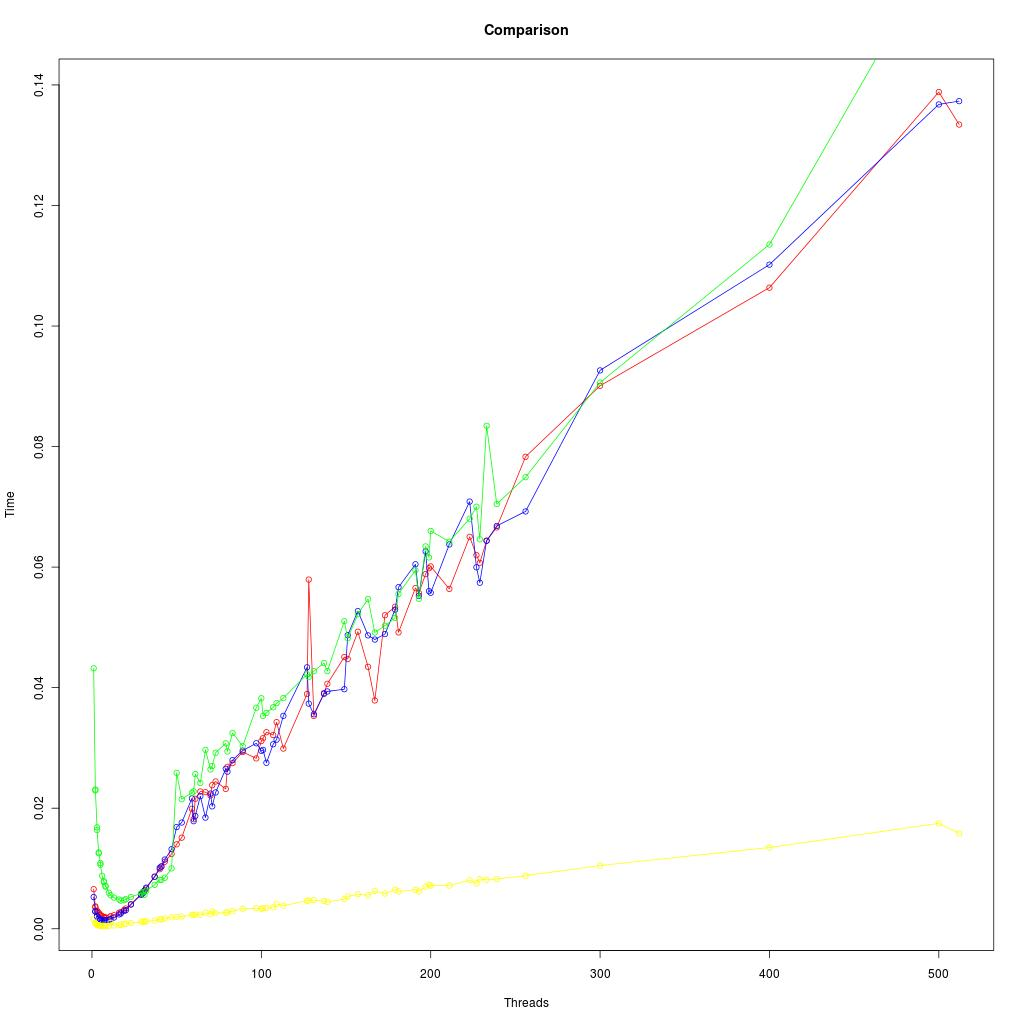
\includegraphics[scale=0.4]{candidate-graphs/omp_p1_compare_200000.jpg}
\end{figure}

\begin{figure}[H]
\centering
\caption{OMP: Comparison of Algorithms at n=10'000. Red = Recursive, Blue = Iterative, 
Green = Hillis-Steele, Yellow = Total Sum}

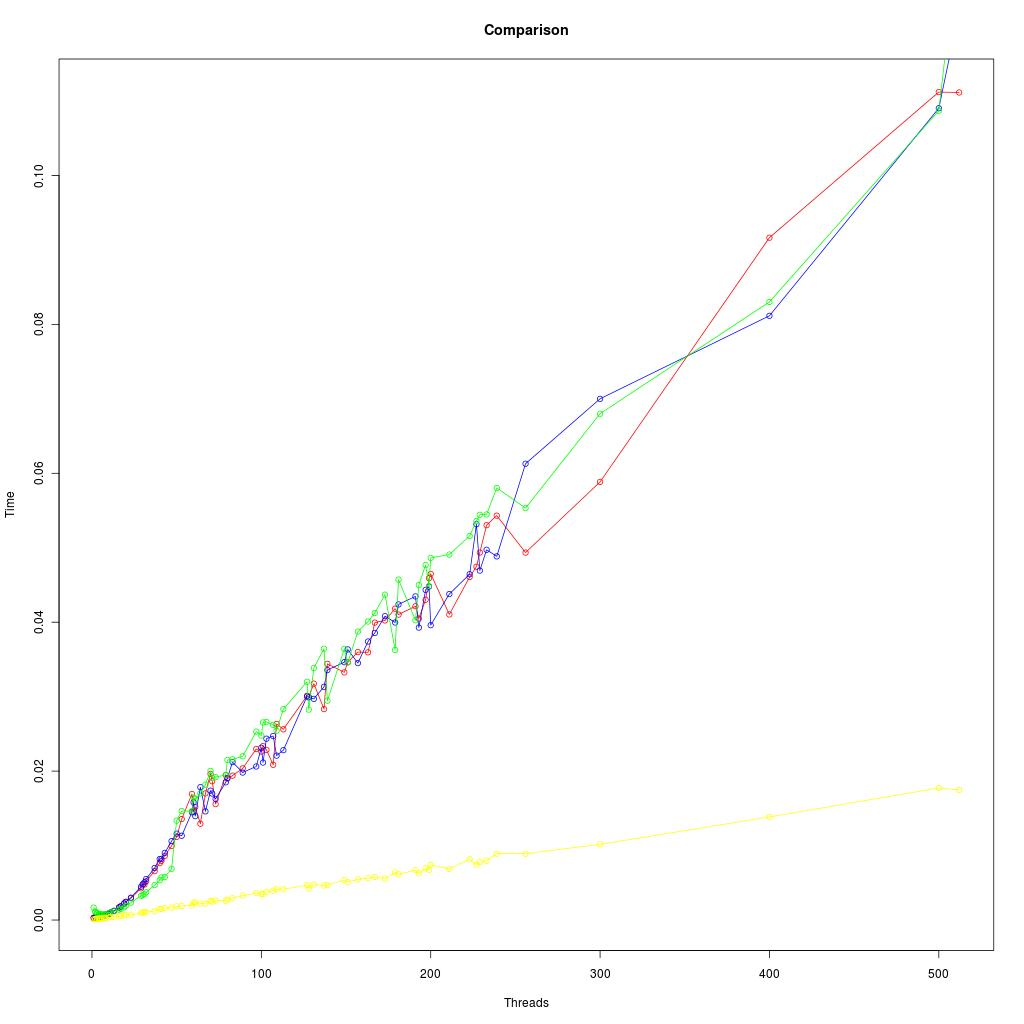
\includegraphics[scale=0.4]{candidate-graphs/omp_p1_compare_10000.jpg}
\end{figure}

\begin{figure}[H]
\centering
\caption{OMP: Comparison of Algorithms at n=256. Red = Recursive, Blue = Iterative, 
Green = Hillis-Steele, Yellow = Total Sum}

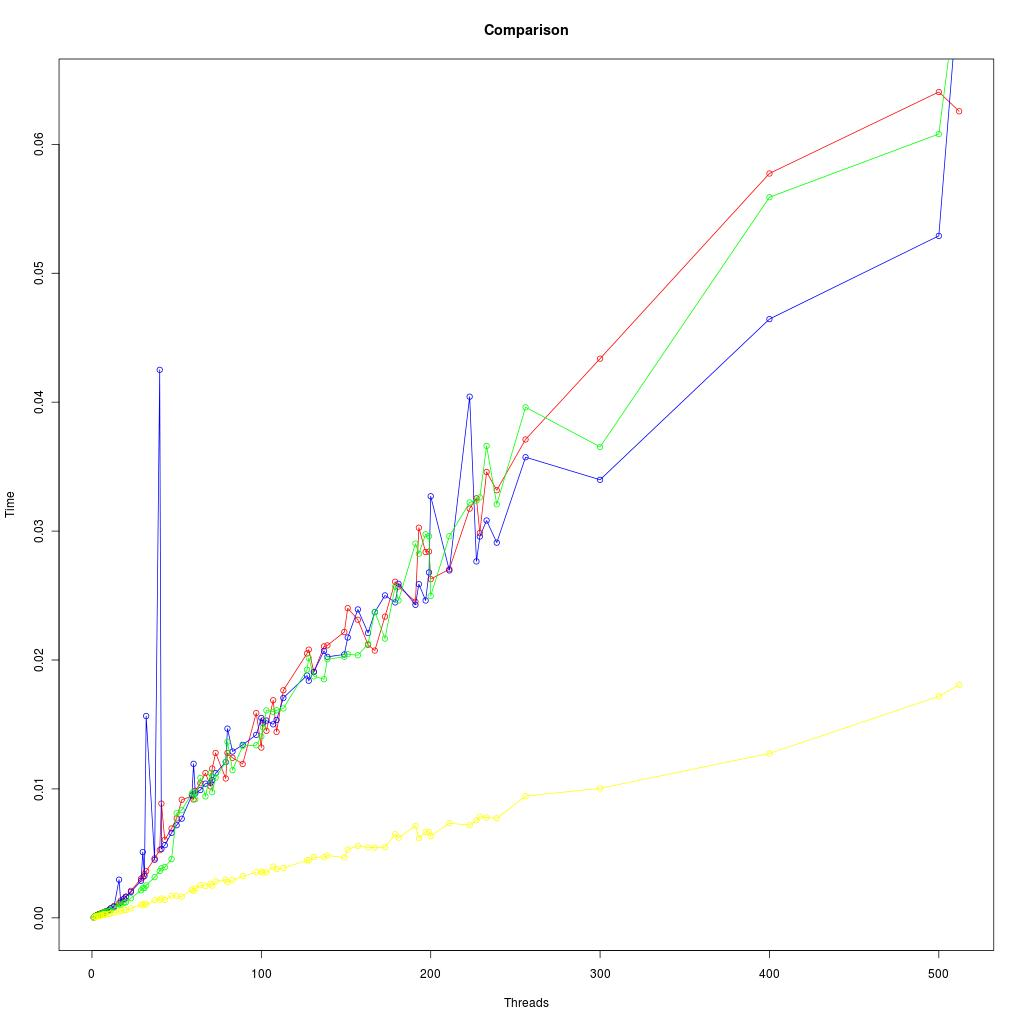
\includegraphics[scale=0.4]{candidate-graphs/omp_p1_compare_256.jpg}
\end{figure}

\begin{figure}[H]
\centering
\caption{OMP: Iterative Algorithm. Fixed Number of Threads (2000)}

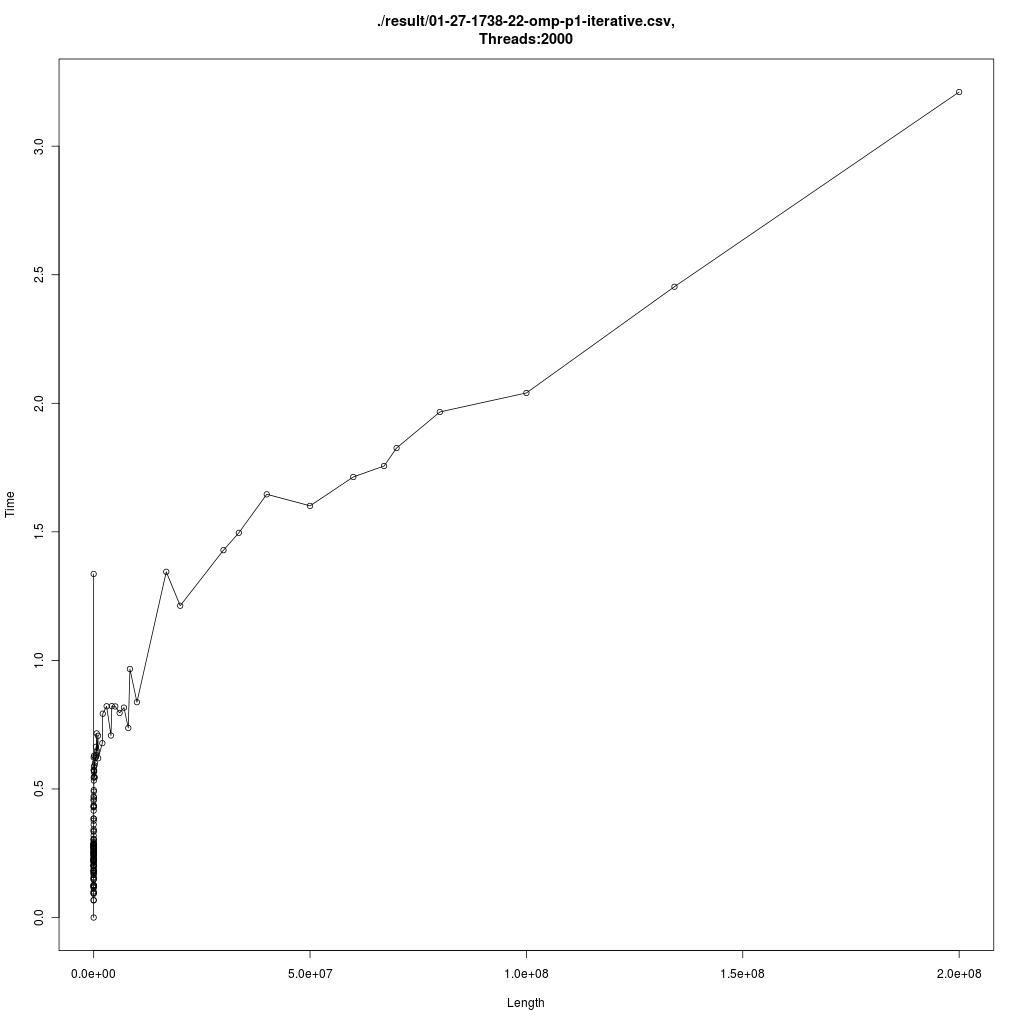
\includegraphics[scale=0.4]{candidate-graphs/omp_p1_iterative_length_2000.jpg}
\end{figure}

\begin{figure}[H]
\centering
\caption{OMP: Sequential Algorithm. Fixed Number of Threads (1)}

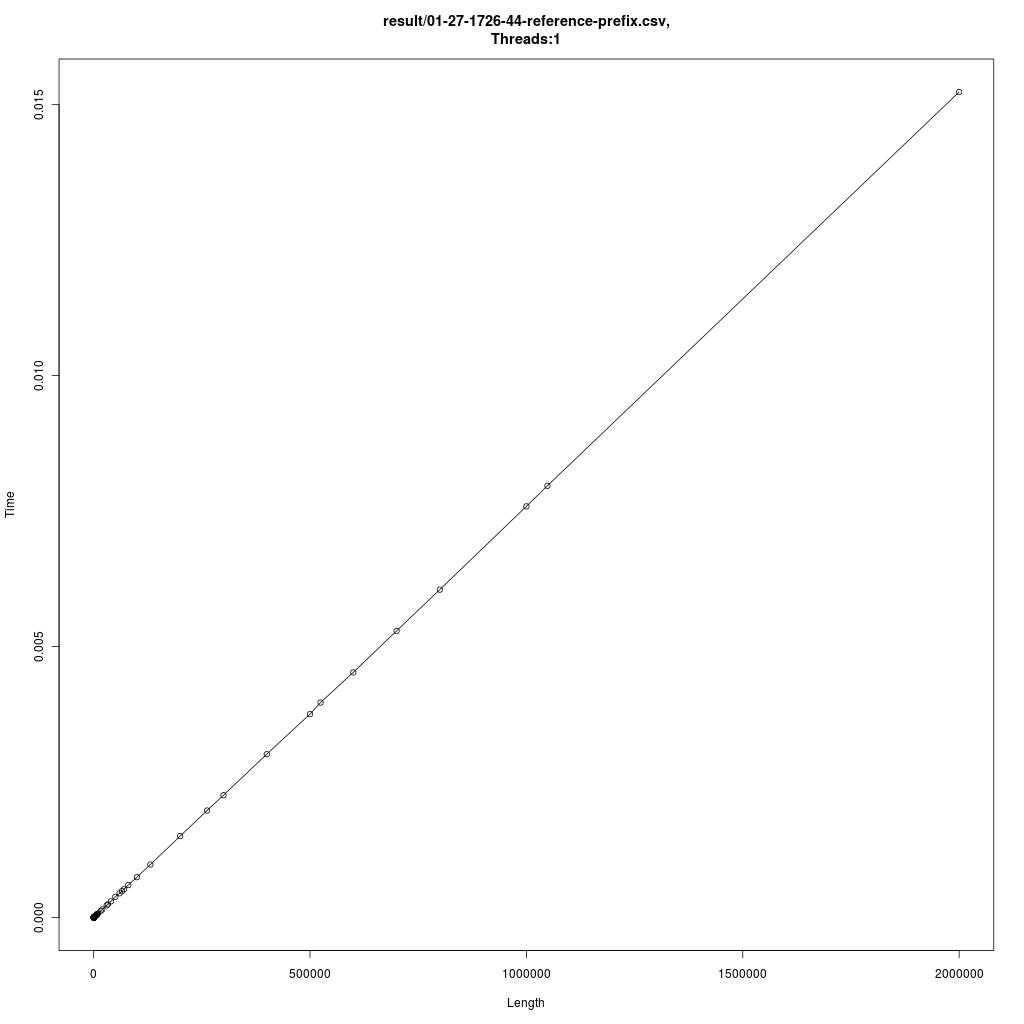
\includegraphics[scale=0.4]{candidate-graphs/omp_p1_length_time_1_XYZ.jpg}
\end{figure}

\newpage
\section{OpenMP: Matrix / Vector Multiplication}
This implementation was also done in OpenMP rather than using pthreads. When calling the program, a tuple $(n, m, t)$ is required to set the dimensions of the matrix and the vector, as well as the amount of threads that should be used to calculate the problem. Invalid input (negative threads, sizes) concludes the program with a message.
Once given adequate input, the program generates a matrix \& vector based on the transmitted size dimensions, once more using \emph{modulo} operations.

The implementation of the algorithm is located in figure \ref{omp_matmult_code}.

Our observations (please see graphs below) have shown that certain column sizes are affected by false sharing (X, Y, Z). For \verb=schedule(static, 1)= (One row per thread), we found XYZ.


\begin{figure}[H]
\label{omp_matmult_code}
\caption{Matrix / Vector Multiplication in OMP}
\begin{lstlisting}
static void matmult(ATYPE mat[], ATYPE vec[], ATYPE* res, int m, int n)
{
	int i, j;

	#pragma omp parallel for schedule(static,1)
	for (i = 0; i < m; i++) 
	{
		res[i] = 0;
		for (j = 0; j < n; j++) 
		{
			// MINDEX returns value of A_(i, j)
			res[i] += mat[MINDEX(i,j)] * vec[j];
		}
	}
}
\end{lstlisting}
\end{figure}

\begin{figure}[H]
\centering
\caption{OMP: Prefix Sums Performance}

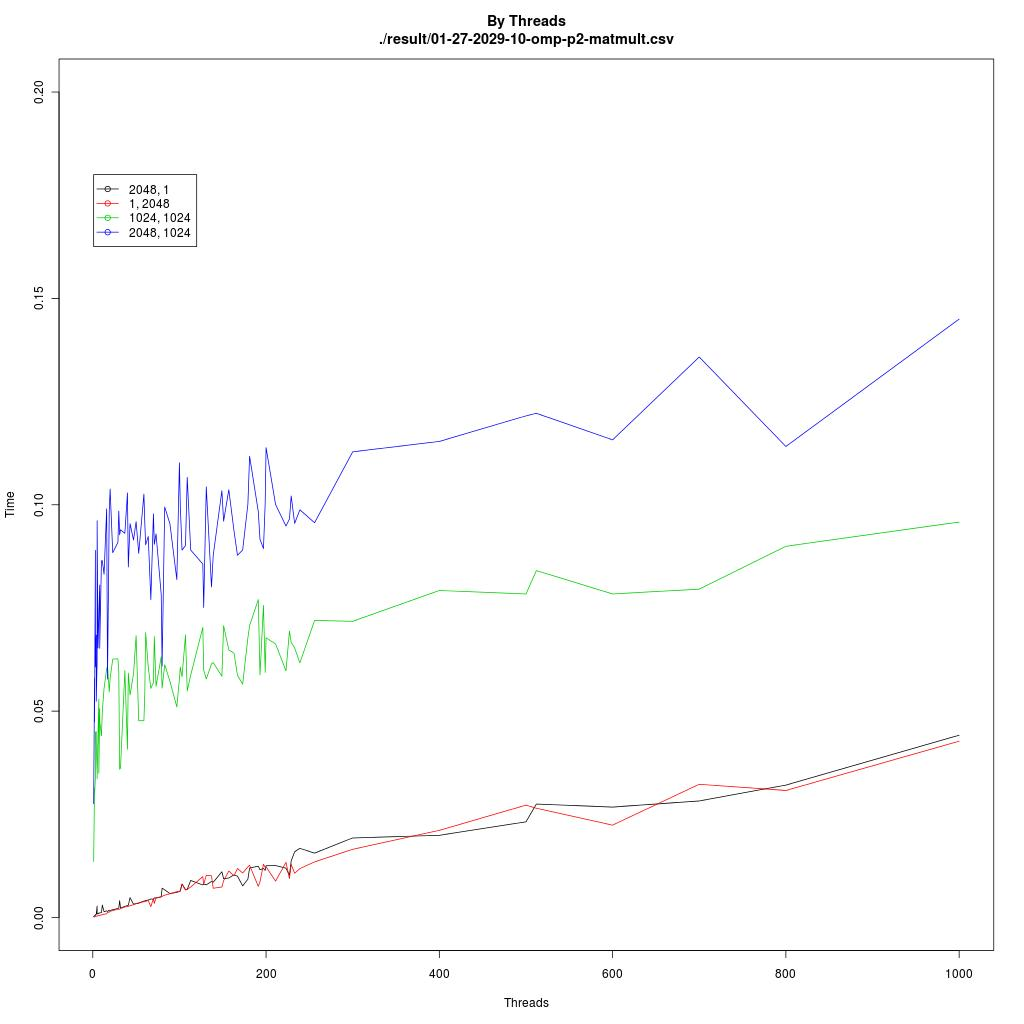
\includegraphics[scale=0.3]{candidate-graphs/omp_p2_fixed_size_16.jpg}
\end{figure}


\newpage
\section{Cilk: Task-parallel Prefix-Sums}
We elected to implement the prefix-sum project for the Cilk category due to the experience gained with the OMP implementations. Again the program requires an input of $n, c, t$ to determine the \emph{total size}, \emph{chunk size} and the number of threads (of course exiting on invalid input). The code in figure \ref{cilk_prefix_code} shows the core of the implemented algorithm.

During the implemmentation, we encountered several challenges with regards to segmentation faults, arising due to calls to C's \verb=alloca=. The calls were replaced by Cilk's own implementation of this functionality (thread-safe): \verb=Cilk_alloca=.

The task parallel ($c > 1$) performance was observed to be vastly superior to data parallel runs. These findings are largely independent of input size $n$ and thread count $t$.

Speed up (in Cilk) (compared OMP \& MPI)



\begin{figure}[H]
\label{cilk_prefix_code}
\caption{Task-parallel Prefix-Sums in Cilk}
\begin{lstlisting}
cilk static void scan(ATYPE* in, int length, int chunk)
{
	int start;
	int count;
	int half;
	ATYPE* out;

	if (length <= 1) return;

	half = length/2;
	out = Cilk_alloca(sizeof(ATYPE) * half);

	for (start = 0; start < half; start += chunk) 
	{
		count = chunk;
		if (start + chunk > half) count = half-start;

		spawn add_up(in, out, start, count);
	}
	sync;

	spawn scan(out, half, chunk);
	sync;

	in[1] = out[0];

	for (start = 1; start < half; start += chunk) 
	{
		count = chunk;
		if (start + chunk > half) count = half-start;

		spawn reduce_down(in, out, start, count);
	}
	sync;

	if (length % 2)
	{
		in[length-1] = out[half-1] + in[length-1];
	}
}
\end{lstlisting}

\end{figure}

\begin{figure}[H]
\centering
\caption{Cilk: Prefix Sum Performance, n=500}

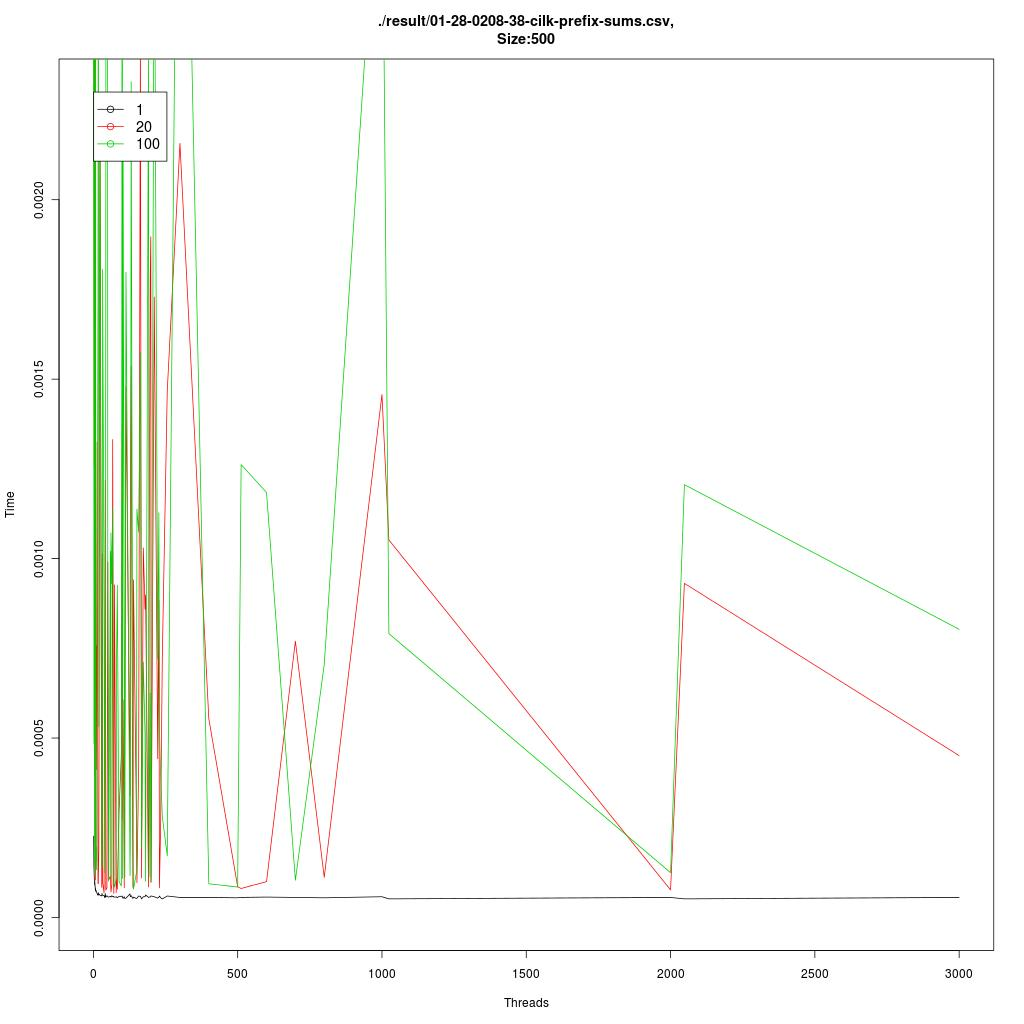
\includegraphics[scale=0.3]{candidate-graphs/cilk_by_threads_500.jpg}

\end{figure}

\begin{figure}[H]
\centering
\caption{Cilk: Prefix Sum Performance, n=10'000}

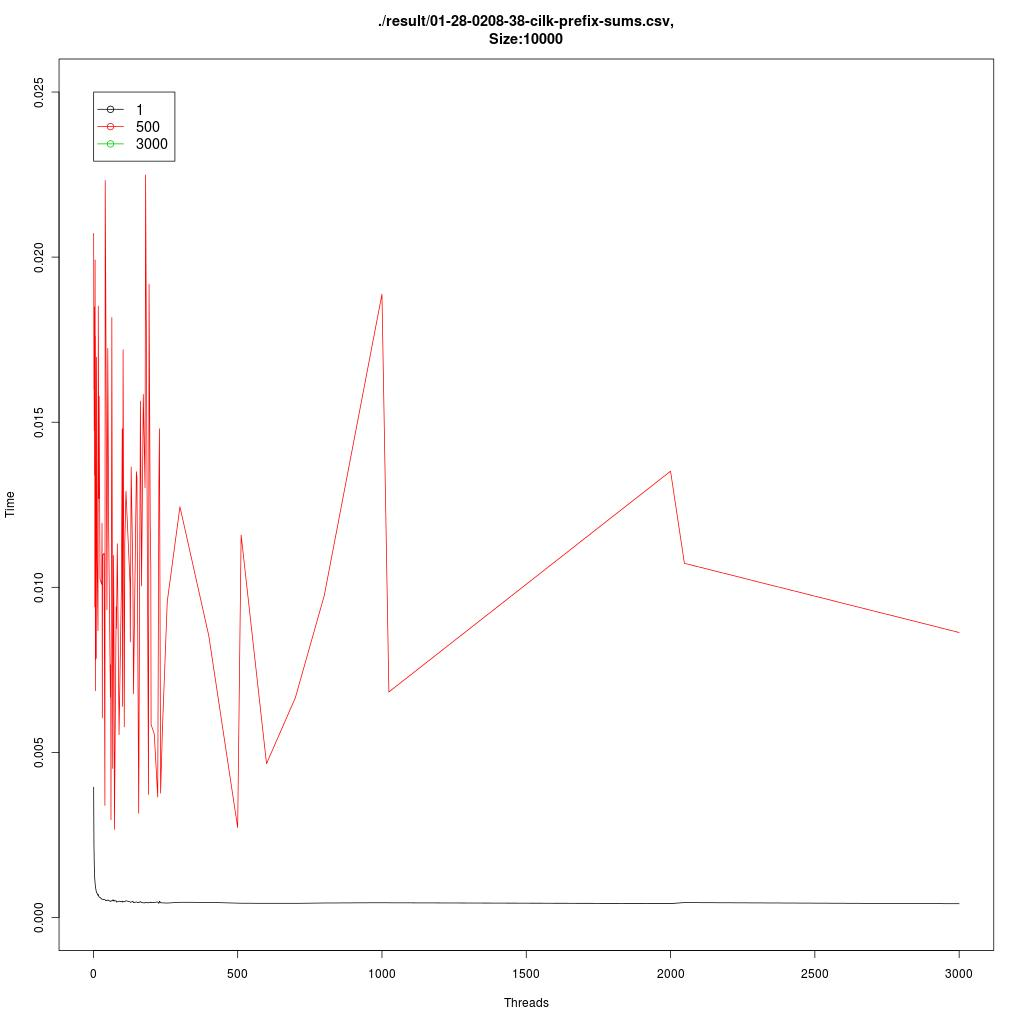
\includegraphics[scale=0.3]{candidate-graphs/cilk_by_threads_10000.jpg}

\end{figure}

\begin{figure}[H]
\centering
\caption{Cilk: Prefix Sum Performance, n=20'000}

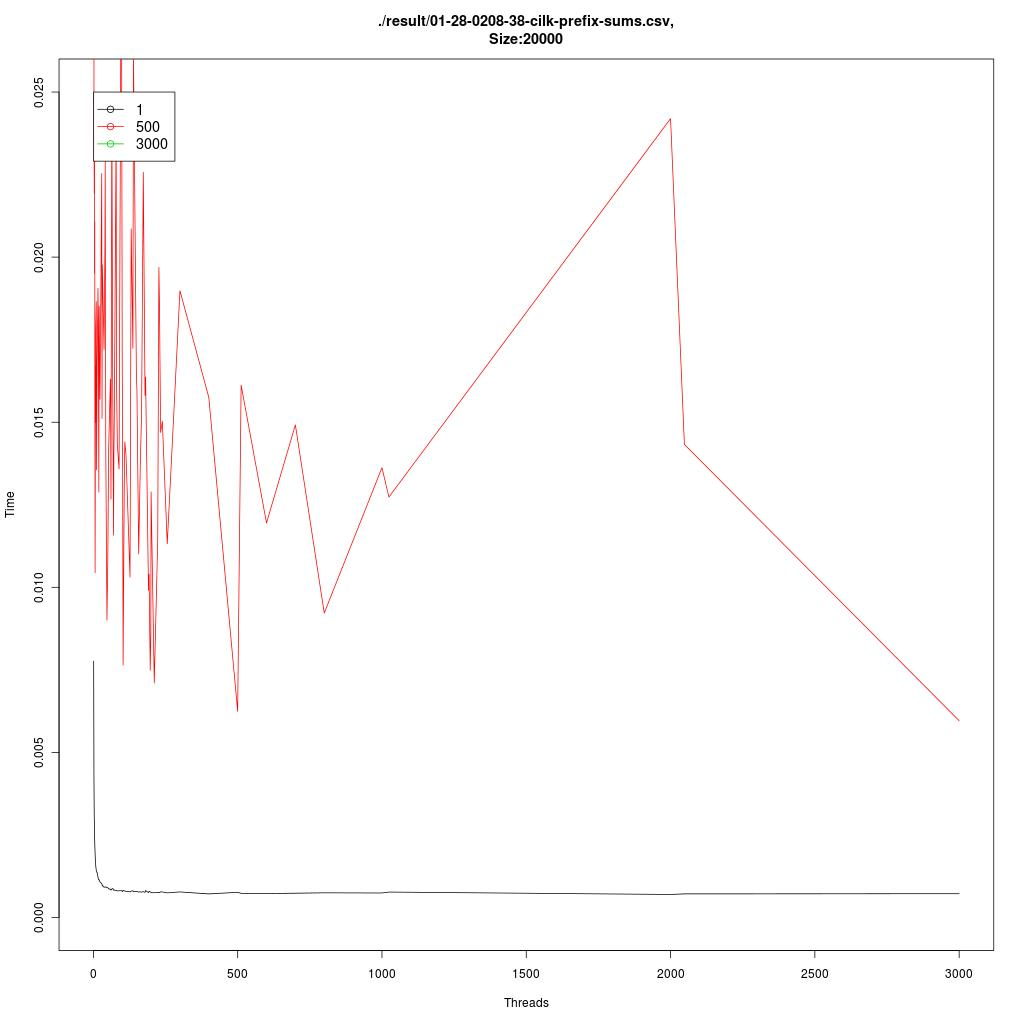
\includegraphics[scale=0.3]{candidate-graphs/cilk_by_threads_20000.jpg}

\end{figure}


\newpage
\section{MPI: Stencil Operations}
The stencil operation was first implemented and tested locally using \emph{OpenMPI} 32-Bit, then re-compiled using \emph{NECmpi} 64-Bit on Jupiter. Instead of using \verb=MPI_Send= or \verb=MPI_Recv=, we opted to use the non-blocking \verb=MPI_ISend= and \verb=MPI_IRecv=. The reasoning behind this approach is that the program can compute the local center of the submatrix while waiting for processes to exchange data concerning the external ring, leading to more efficient use of the CPU and idle times.

Based on data, we estimate that the running time can be calculated as follows (please see figure \ref{mpi_stencil_code} for code extract):

\begin{eqnarray}
C_{par} \cdot \left( \max(T_{StencilMid}, T_{Comm}) + T_{StencilRing} \right)\\
C_{par} = O\left(\max(\frac{r\cdot c}{p}, 1)\right)\\
T_{StencilMid} = O\left(\frac{m}{c} \cdot \frac{n}{r}\right)\\
T_{Comm} = O\left(\frac{m}{r} + \frac{n}{c}\right)\\
T_{StencilRing} = O\left(\frac{m}{r} + \frac{n}{c}\right)
\end{eqnarray}

$C_{par}$ is a factor that increases the required time, depending on whether enough cores are available to distribute the $(r \cdot c)$ work blocks evenly and process them all in parallel. If not enough cores are available, the time increases. $T_{StencilMid}$ is the time needed to calculate the stencil values for the center cells of a submatrix (where no communication with other processes is required) and $T_{Comm}$ represents the time needed to communicate the data with neighboring processes. $T_{StencilRing}$ is the time required to run remaining stencil calculations after new data has been received.

To achieve maximum parallellization under this model, we should choose $r$ and $c$ in a way so that $rc = p$, leading to the lowest $C_{par} = 1$. We can now consider the following scenarios:

\begin{enumerate}
\item (Block format) $r = c = \sqrt{p}$ 
\item (Column Format) $r = 1, c = p$
\item (Row Format) $r = p, c = 1$
\end{enumerate}

We can conclude that $T_{StencilMid}$ is not affected by the choice of $r$ and $c$, since $p = rc$, leading to $O(\frac{mn}{p})$. We therefore aim to minimize $T_{Comm}$ to the point of $T_{Comm} \leq T_{StencilMid}$. Determing which distribution (block vs. column) is optimal could not be determined analytically; empirical data is available.

\begin{figure}[H]
\label{mpi_stencil_code}
\caption{Stencil Operation in MPI}
\begin{lstlisting}
	/*
	  Terminology:
		m: Number of rows in matrix,          e.g. 15
		n: Number of columns in matrix,       e.g. 8
		r: Number of block rows,              e.g. 5
		c: Number of block columns,           e.g. 4
		h: Height (rows) of a single block,   e.g. 3
		w: Width (columns) of a single block, e.g. 2
		i: Block Row index                    (0-4)
		j: Block Column index                 (0-3)
		x: Row index in matrix                (0-14)
		y: Column index in matrix             (0-7)
	 */
	// start indices of this node's submatrix
	x = j * w;
	y = i * h;
	// allocate my submatrix (twice)
	ATYPE* source = xmalloc((w+2) * (h+2) * sizeof(ATYPE));
	ATYPE* dest = xmalloc(w * h * sizeof(ATYPE));
	genmatrix(source, x, y, w, h, n);

	int ret;
	MPI_Request request[8];
	MPI_Datatype column_type;
	MPI_Type_vector(h, 1, w+2, ATYPE_MPI, &column_type);
	MPI_Type_commit(&column_type);

	int l_peer = rank-1; if (j <= 0)   l_peer = MPI_PROC_NULL;
	int r_peer = rank+1; if (j >= c-1) r_peer = MPI_PROC_NULL;
	int u_peer = rank-c; if (i <= 0)   u_peer = MPI_PROC_NULL;
	int d_peer = rank+c; if (i >= r-1) d_peer = MPI_PROC_NULL;

	ret = MPI_Isend(&source[(w+2)+1],       1, column_type, l_peer, LEFT,  MPI_COMM_WORLD, &request[0]);
	ret = MPI_Isend(&source[(w+2)+w],       1, column_type, r_peer, RIGHT, MPI_COMM_WORLD, &request[1]);
	ret = MPI_Isend(&source[(w+2)+1],       w, ATYPE_MPI,   u_peer, UP,    MPI_COMM_WORLD, &request[2]);
	ret = MPI_Isend(&source[h*(w+2)+1],     w, ATYPE_MPI,   d_peer, DOWN,  MPI_COMM_WORLD, &request[3]);

	ret = MPI_Irecv(&source[(w+2)],         1, column_type, l_peer, RIGHT, MPI_COMM_WORLD, &request[4]);
	ret = MPI_Irecv(&source[(w+2)+w+1],     1, column_type, r_peer, LEFT,  MPI_COMM_WORLD, &request[5]);
	ret = MPI_Irecv(&source[1],             w, ATYPE_MPI,   u_peer, DOWN,  MPI_COMM_WORLD, &request[6]);
	ret = MPI_Irecv(&source[(h+1)*(w+2)+1], w, ATYPE_MPI,   d_peer, UP,    MPI_COMM_WORLD, &request[7]);

	stencil_middle(source, dest, w, h);
	ret = MPI_Waitall(8, request, MPI_STATUS_IGNORE);
	stencil_ring(source, dest, w, h);

\end{lstlisting}
\end{figure}


\newpage
\section{MPI: Prefix Sums}
The algorithm was implemented using the \verb=MPI_Sendrecv= to realize the \emph{Hillis-Steele} algorithm with communication.The implemented algorithm differs from MPI's standard algorithm in that MPI's version allows for further consideration of nodes / ranks with regard to influencing factors such as locality, which the presented algorithm does not take into account.

We have established correctness of the algorithm via integrated reference function and also other project results (see OMP).

The running time of the algorithm $R(n, p)$ is calculated as below, given the following assumptions:
\begin{enumerate}
\item The network throughput is constant, i.e. there is no network congestion. Two communicating nodes can always transmit data at constant speed.
\item $T_{comm}$ shows linear growth relative to the amount of data to be transmitted.
\end{enumerate}

\begin{eqnarray}
T_{par} = T_{Iteration} * Iterations\\
Iterations = O(\log n)\\
T_{Iteration} = T_{comm} + T_{ops}\\
T_{comm} = O\left(\frac{n}{p}\right)\\
T_{ops} = O\left(\frac{n}{p}\right)
\end{eqnarray}

Observations reveal that a speed-up of XYZ relative to sequential reference implementation of the prefix sum algorithm was achieved (see empirical data).

\begin{figure}[H]
\label{mpi_prefix_code}
\caption{Prefix sum in MPI}
\begin{lstlisting}
static void dist_sum(int rank, int p, ATYPE b, ATYPE* prefix)
{
	ATYPE buf;
	*prefix = 0;

	for (int k = 1; k < p; k<<=1) 
	{
		int rpeer = rank - k;
		int speer = rank + k;

		if (speer >= p)
		{
			speer = MPI_PROC_NULL;	
		}

		if (rpeer < 0)
		{
			buf = 0;
			rpeer = MPI_PROC_NULL;
		}

		int ret = MPI_Sendrecv(&b, 1, ATYPE_MPI, speer, k, &buf, 1, ATYPE_MPI, rpeer, k, MPI_COMM_WORLD, MPI_STATUS_IGNORE);
		
		*prefix += buf;
		b += buf;
	}
}
\end{lstlisting}

\end{figure}

\newpage
\section{MPI: Matrix / Vector Multiplication}
Both the \verb=MPI_Allgather= and \verb=MPI_Reduce_scatter= algorithms were used alongside a regular sequential reference implementation to calculate speedup relations. Testing was done using already existing infrastructure from previous projects. The implementation makes no restrictions on the dimensions; specifically, the generated matrix does not need to be square for the algorithm to work. However, the program does require that both matrix dimensions are divisible by $p$ (if not, error message is given).


\end{document}
